\documentclass{article}

\usepackage{../parm}
\begin{document}

    \section{Présentation du projet}

    \subsection{Le microprocesseur ARM Cortex-M0}

    La famille des ARM Cortex-M regroupe des processeurs 32 bits.
    Ils peuvent être utilisés comme microprocesseur ou microcontrôleur.
    On les retrouve dans diverses applications : Arduino Due, machine à laver, distributeur de boissons... Les Cortex-M visent en majorité le marché de l'embarqué.

    Le but de ce projet est de simuler le comportement d'un Cortex-M0 au moyen d'un logiciel de simulation électronique: \texttt{Logisim}.
    L'idée est ici d'obtenir un système ayant un comportement similaire à un Cortex-M0 et non une copie conforme du fait de la complexité d'un processeur réel.

    \subsection{Le projet}
    Durant ce projet nous allons implémenter notre microprocesseur en le divisant en plusieurs blocs:
    \begin{itemize}
        \item Partie matérielle:
        \begin{itemize}
            \item ALU 32 bits
            \item Banc de 8 registres
            \item Contrôleur
        \end{itemize}
        \item Partie logicielle:
        \begin{itemize}
            \item Assembleur
            \item Exportation sur FPGA
        \end{itemize}
    \end{itemize}

    \paragraph{Spécificités de l'implémentation}
    \begin{itemize}
        \item Pas de gestion des interruptions
        \item Pas de gestion des appels de fonctions
        \item Pas d'optimisation
        \item Pas de pipeline
        \item Pas de FPU \footnote{\textit{Floating-Point Unit}, unité de calcul en virgule flottante}
        \item Pas de MMU \footnote{\textit{Memory Management Unit}, unité de gestion mémoire, gère la traduction des adresses virtuelles en adresses physiques au sein du processeur}
        \item Toutes les instructions s'exécutent en 1 cycle (excepté les instructions \texttt{LDR}/\texttt{STR} en 2 cycles)
        \item Instructions sur 16 bits
        \item Données sur 32 bits
        \item Adressage RAM/ROM sur 9 bits
        \item Adressage RAM uniquement sur la pile (en utilisant le \textit{Stack Pointer})
    \end{itemize}

    \subsection{Logisim}

    \texttt{Logisim} est un programme permettant la modélisation et la simulation de circuit logique.
    La modélisation du circuit ne se fait que par dessin et glisser-déposer des différents éléments électroniques.

    \paragraph{Installation:} la version de \texttt{Logisim} utilisé dans le cadre du projet est la 3.5.0, accessible à l'adresse \url{https://github.com/logisim-evolution/logisim-evolution/releases/tag/v3.5.0}.
    Sur Windows, utilisez le fichier \texttt{.msi} pour installer.
    Sur Mac, utilisez le fichier \texttt{.dmg}.
    Sur Ubuntu/Debian, passez par le fichier \texttt{.deb} avec la commande :
    \begin{lstlisting}
sudo apt install gdebi
sudo gdebi logisim-evolution_3.5.0-1_amd64.deb
    \end{lstlisting}
    Pour les autres systèmes, vous pouvez lancer directement le fichier .jar sans installer. La commande à utiliser est :
    
    \begin{lstlisting}[language=bash]
java -Dsun.java2d.opengl=true -jar logisim-evolution.jar
    \end{lstlisting} 

    \textit{Cette section est un extrait du tutoriel officiel «Introduction à l’utilisation de Logisim». Pour plus d'informations, se référer à la documentation officielle.}

    Vous pouvez voir l'interface de \texttt{Logisim} sur la Figure  \ref{fig_logisim_description}.

    \begin{figure}[t]
        \begin{center}
            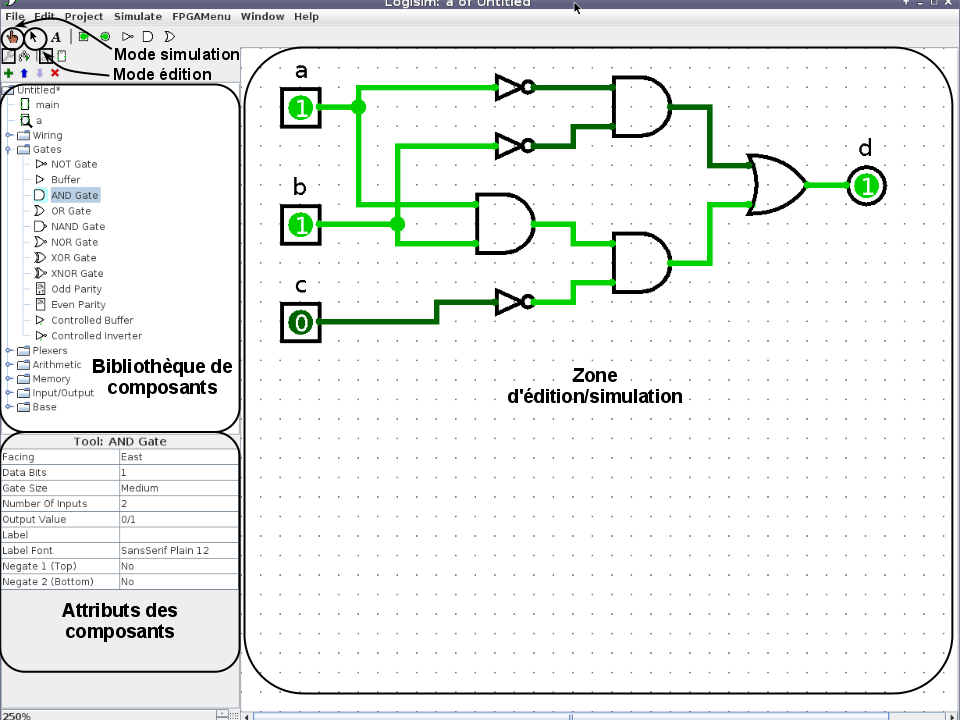
\includegraphics[width=500pt]{pictures/Logisim_description.png}
            \caption{\label{fig_logisim_description}Interface de Logisim}
        \end{center}
    \end{figure}

    Une des particularités de \texttt{Logisim} est de pouvoir éditer et simuler un circuit en même temps.
    Nous expliquerons plus tard dans ce document comment simuler un circuit, puis comment l'implémenter sur la carte du
    laboratoire.


%%%%%%%%%%%%%%%%%%%%%%%%%%%%%%%%%%%%%%%%%%%%%%%%%

    \subsubsection{Mode édition}
    \begin{enumerate}
        \item Pour utiliser le mode édition, il faut simplement sélectionner la flèche comme indiqué en haut de la figure
        \ref{fig_logisim_description}.
        \item On peut alors choisir un composant dans la bibliothèque sur la gauche.
        Pour l'ajouter dans son schéma, il suffit
        de cliquer sur le composant désiré, puis de cliquer sur le schéma.

        \item Chaque composant que vous utiliserez aura des attributs modifiables dans la zone inférieur gauche de
        \texttt{Logisim}.
        Par exemple si l'on pose une porte \texttt{AND}, on peut modifier le nombre de signaux qu'elle prend en
        entrée, ou encore mettre un inverseur sur une de ses entrées.

        \item Il est aussi possible de faire des copier/coller d'un ou plusieurs composants.
        Dans ce cas, les composants
        conserverons aussi tous les attributs préalablement définis.

        \item Une fois que l'on a posé tous les composants, il faut alors les connecter.
        Pour cela il suffit de placer le curseur
        avec la souris sur un des ports à connecter et, en gardant pressé le bouton
        gauche de la souris, le déplacer jusqu'au port de destination.

    \end{enumerate}

%%%%%%%%%%%%%%%%%%%%%%%%%%%%%%%%%%%%%%%%%%%%%%%%%

    \subsubsection{Création d'un premier circuit}



    \label{nouveauCircuit}
    Tous les circuits réalisés dans \texttt{Logisim} peuvent être réutilisés dans d'autres circuits.
    Afin de créer un nouveau circuit, il faut aller dans \texttt{Projet} $\rightarrow$ \texttt{Ajouter Circuit...} et nommer le circuit.
    Le circuit créé devient un composant disponible dans la bibliothèque.

%%%%%%%%%%%%%%%%%%%%%%%%%%%%%%%%%%%%%%%%%%%%%%%%%

    \subsubsection{Mode simulation}
    \texttt{Logisim} est capable de simuler le circuit en affichant les valeurs des signaux directement sur le schéma.
    L'utilisateur
    peut alors définir les valeurs des bits en entrée et observer la réaction du design.
    \begin{enumerate}
        \item Pour utiliser le mode simulation, il faut sélectionner la main en haut à gauche de \texttt{Logisim} (cf
        Figure~\ref{fig_logisim_description})

        \item Il est alors possible de contrôler l'état des différentes entrées en cliquant directement dessus.

        \item En cliquant sur une entrée, la valeur doit alterner entre \texttt{0} ou \texttt{1}.

        \item Voici un descriptif des couleurs utilisées pour les signaux en mode simulation.
        \begin{figure}[H]
            \begin{center}
                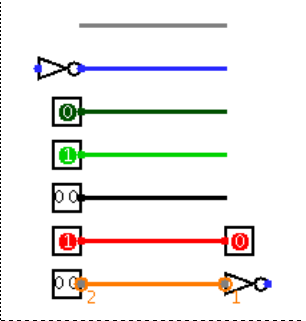
\includegraphics[scale=0.4]{pictures/logisim_couleurs.png}
                \caption{\label{fig_logisim_couleur}Couleurs des fils en simulation}
            \end{center}
        \end{figure}

        \begin{itemize}
            \item \textbf{Gris}: La taille du fil est inconnue.
            Le fil n'est relié à aucune entrée ou sortie.
            \item \textbf{Bleu}: Le fil comporte une valeur, cependant elle est inconnue.
            \item \textbf{Vert foncé}: Le fil comporte la valeur \texttt{0}.
            \item \textbf{Vert clair}: Le fil comporte la valeur \texttt{1}.
            \item \textbf{Noir}: Le fil comporte plusieurs bits (bus).
            \item \textbf{Rouge}: Le fil comporte une erreur.
            \item \textbf{Orange}: Les composants reliés au fil n'ont pas la bonne taille.
        \end{itemize}

    \end{enumerate}

%%%%%%%%%%%%%%%%%%%%%%%%%%%%%%%%%%%%%%%%%%%%%%%%%

    \subsubsection{Design hiérarchique}
    La méthodologie de design que l'on vient d'utiliser est valable pour la conception de systèmes numériques plutôt
    simples, c'est-à-dire avec un nombre de portes logiques plutôt bas.
    Lorsque l'on vise des systèmes plus compliqués on
    risque de voir le nombre de portes et de connexions exploser.
    Dans ce cas, le risque d'introduire des erreurs devient
    très important.

    La clé pour gérer correctement une complexité plus grande est d'utiliser le design hiérarchique.
    Grâce au design
    hiérarchique on peut travailler à différents niveaux d'abstraction.
    D'abord on décrit des blocs de base à l'aide des
    portes logiques, pour ensuite utiliser ces blocs de base comme parties d'un système plus large.

    Pour créer un design hiérarchique il faudra suivre les pas
    suivants:
    \begin{enumerate}
        \item Créez un nouveau circuit comme déjà expliqué dans la section \ref{nouveauCircuit} et nommez le.
        Pour passer de l'édition d'un circuit à l'autre, il suffit de double-cliquer sur le nom de celui désiré dans le menu de
        gauche.
        \item Il est alors possible d'ajouter un sous circuit de la même manière que l'utilisation d'un
        composant quelconque.
        On clique sur le sous circuit en question dans le menu indiqué sur la Figure~\ref{fig_sousCircuit}, puis on le
        place en cliquant sur la zone d'édition.
        \item Si le sous circuit avait été créé correctement, alors il devrait être représenté par un petit bloc, avec
        sur sa gauche des points bleus correspondant aux entrées, et sur sa droite des points verts correspondant aux sorties.
        \item Si les sorties apparaissent en bleu et non en vert sur le schéma, vérifiez que vous avez bien affecté l'attribut
        \texttt{Sortie?} $=$ \texttt{Oui} dans les \texttt{Pin}s de sortie.

    \end{enumerate}

    \begin{figure}[H]
        \begin{center}
            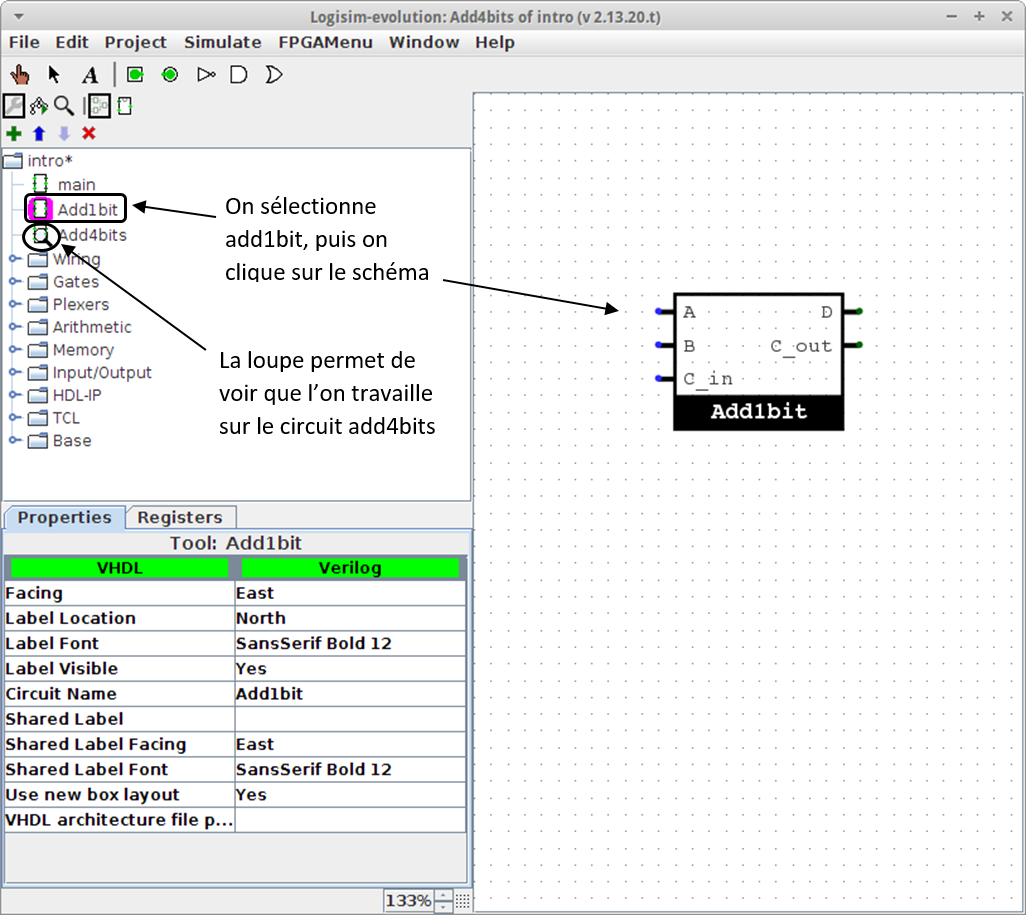
\includegraphics[width=450pt]{pictures/logisim_sousCircuit.png}
            \caption{\label{fig_sousCircuit}Sous circuit}
        \end{center}
    \end{figure}

    \subsubsection{Bus et séparateurs}

    Pour l'implémentation de composant travaillant avec des données sur plusieurs bits (un additionneur par exemple),
    il devient nécessaire de regrouper plusieurs signaux en créant un bus de données.
    Par exemple, pour définir l'entrée A comme un bus de 4 bits, il
    faut ajouter un élément \texttt{Pin} et définir sa taille via l'attribut \texttt{Data bits} $=$ \texttt{4}.

    Lorsque l'on tire un fil de l'une de ces entrées, ce n'est plus un simple signal mais un bus de 4 bits.
    Pour
    pouvoir connecter les éléments de ce bus aux entrées de plusieurs composants travaillant sur chacun un bit,
    on va devoir séparer les différents fils du bus afin de pouvoir les traiter un par un.
    L'élément \texttt{Séparateur}
    de \texttt{Cablage} permet d'effectuer ces conversions dans les deux sens: d'un bus de 4 bits vers 4 fils,
    et de 4 fils vers un bus de 4 bits -- voir Figure~\ref{fig_splitter}.

    \begin{figure}[H]
        \begin{center}
            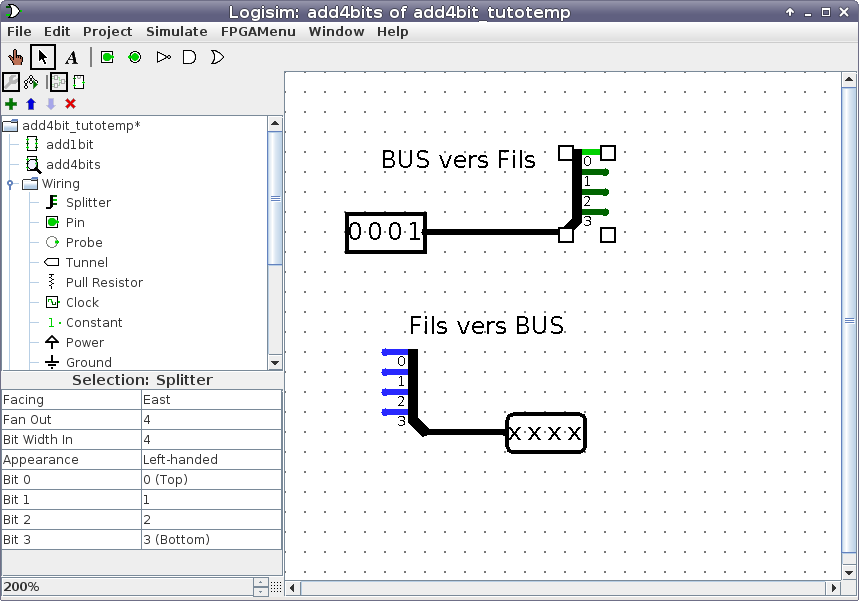
\includegraphics[width=500pt]{pictures/logisim_splitters.png}
            \caption{\label{fig_splitter}Exemples splitters}
        \end{center}
    \end{figure}

    Il faut définir les tailles d'entrées et de sorties du \texttt{Séparateur} via les attributs \texttt{Ventilation en sortie} et
    \texttt{Largeur de bits en entrée}.

    \paragraph{Note:} le bit de poids faible est indexé à 0 en sortie du \texttt{splitter}.

    \paragraph{Remarque:} n'utiliser que des composants dont l'indicateur \texttt{VHDL} dans la zone \texttt{Properties} est vert.
    Les autres (\texttt{Buffer controllé} par exemple) ne pourront pas être déployés sur la carte FPGA.
\end{document}